\documentclass[fleqn]{beamer}

\usetheme{Warsaw}
\usepackage{helvet}

\usepackage{amsmath}
\usepackage[absolute, overlay]{textpos}

% \usepackage[utf8]{inputenc}
\usepackage[english]{babel}
\usepackage[style=ngerman]{csquotes}

\usepackage[T1]{fontenc}
\usepackage{lmodern}
\renewcommand{\familydefault}{lmss}

\usepackage{listings}
\usepackage{amsfonts}
\usepackage{amsmath}
\usepackage{amssymb}
\usepackage{array}
\usepackage{calc}
\usepackage{color}
\usepackage{curves}
\usepackage{fancyhdr}
\usepackage{fancyvrb}
\usepackage{graphicx}
\usepackage{hyperref}
\usepackage{latexsym}

\usepackage{setspace}
\usepackage{textcomp}


\definecolor{gray}{gray}{0.5}
\definecolor{green}{rgb}{0,0.5,0}


\lstnewenvironment{python}[1][]{
\lstset{
language=python,
basicstyle=\ttfamily\small\setstretch{1},
stringstyle=\color{red},
showstringspaces=false,
alsoletter={1234567890},
otherkeywords={\ , \}, \{},
keywordstyle=\color{blue},
emph={access,and,break,class,continue,def,del,elif,else,%
except,exec,finally,for,from,global,if,import,in,is,%
lambda,not,or,pass,print,raise,return,try,while},
emphstyle=\color{black}\bfseries,
emph={[2]True, False, None, self},
emphstyle=[2]\color{green},
emph={[3]from, import, as},
emphstyle=[3]\color{blue},
upquote=true,
morecomment=[s]{"""}{"""},
commentstyle=\color{gray}\slshape,
literate=*{:}{{\textcolor{blue}:}}{1}%
	{=}{{\textcolor{blue}=}}{1}%
	{-}{{\textcolor{blue}-}}{1}%
	{+}{{\textcolor{blue}+}}{1}%
	{*}{{\textcolor{blue}*}}{1}%
	{!}{{\textcolor{blue}!}}{1}%
	{(}{{\textcolor{blue}(}}{1}%
	{)}{{\textcolor{blue})}}{1}%
	{[}{{\textcolor{blue}[}}{1}%
	{]}{{\textcolor{blue}]}}{1}%
	{<}{{\textcolor{blue}<}}{1}%
	{>}{{\textcolor{blue}>}}{1},%
frame=lines,#1
}\medskip}{\medskip}

%custom commands
\newcommand{\superscript}[1]{\ensuremath{^{\textrm{#1}}}}
\newcommand{\subscript}[1]{\ensuremath{_{\textrm{#1}}}}
\newcommand{\curldoquom}[1]{\textquotedblleft
#1\textquotedblright\hspace{.01mm}}
\newcommand{\pc}[1]{\setcounter{page}{#1}}
\newcommand{\ppc}[1]{\pause\setcounter{page}{#1}}


\beamertemplatenavigationsymbolsempty
\setbeamertemplate{footline}[page number]

\beamertemplatenavigationsymbolsempty

\title[Topology and dynamics in biological neural networks]{Topology and
dynamics in biological neural networks}
\author[Alejandro F. Bujan]{Alejandro F. Bujan, Jyotika Bahuguna}
%\institute[BCF]{Bernstein Center Freiburg}
\date[]{BNN Course, \today}


\AtBeginSection[]
{
  \setbeamertemplate{footline}{}
  \begin{frame}<beamer>{Outline}
  \footnotesize
  \tableofcontents[currentsection,currentsubsection]
  \end{frame}
  \setbeamertemplate{footline}[page number]
  \normalsize
  }


\begin{document}

\begin{frame}
  \titlepage
\end{frame}

{
\setbeamertemplate{footline}{}
\begin{frame}{Outline}
  \footnotesize
  \tableofcontents
  \normalsize
\end{frame}
}

\setcounter{page}{0}

\section{Introduction}





\subsection{Dynamics}
\begin{frame}{Measure of Network dynamics}
  \begin{itemize}
      \item   Firing rate\ppc{2}
      \item  Variability:\ppc{2}
      \begin{itemize}
      \item  Inter-spike intervals (CV)\ppc{2}
      \item  Spike counts (Fano factor)\ppc{2}
      \end{itemize}
      \item  Co-variability:\ppc{2}
	\begin{itemize}
	  %\item Variance of the PSTH (peristimulus time histogram)\ppc{2}
	  \item Pairwise correlations (between pairs of neurons)\ppc{2}
	  \item Higher order correlations (between triplets,
quadruplets,...)\ppc{2}
	  \item Power spectrum (frequency domain)
	\end{itemize}
      \end{itemize}
\end{frame}

\subsection{Random connectivity}

\pc{3}

\begin{frame}{Is random good enough? (I): Cortical activity}
\begin{minipage}{.48\linewidth}
  \begin{center}
  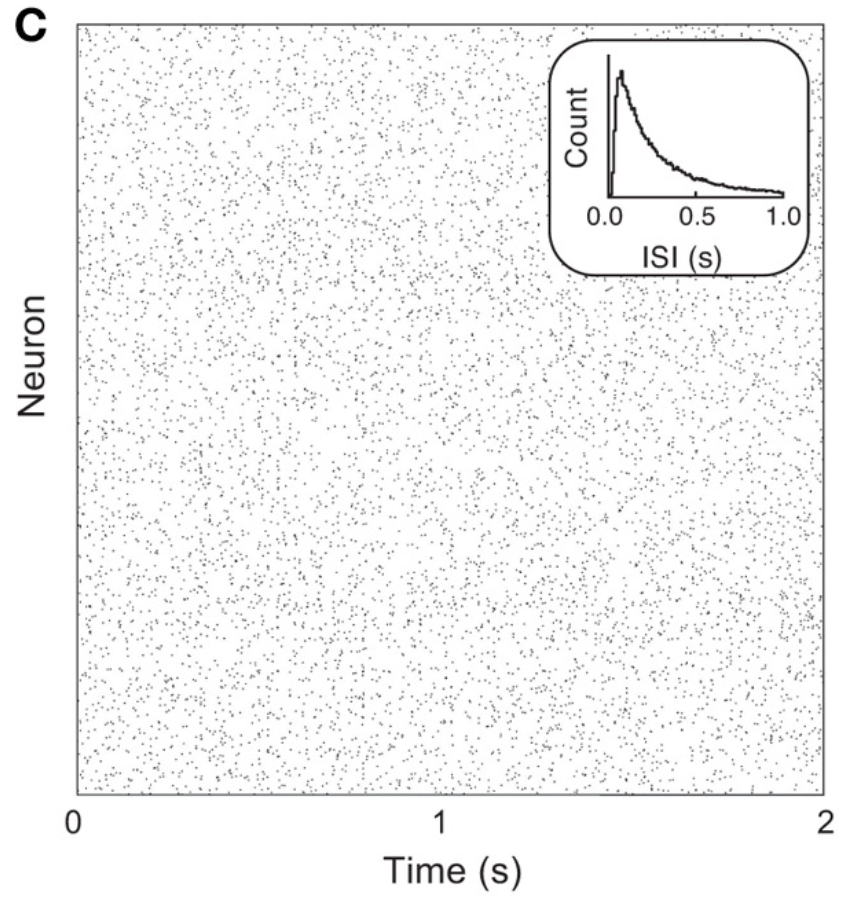
\includegraphics[width=.7\textwidth]{figures/doiron0.png}
  \end{center}
  \begin{flushright}
    {\footnotesize \cite{Doiron2014}}
  \end{flushright}
\end{minipage}\ppc{3}
\begin{minipage}{.48\linewidth}
  Cortical activity in awake behaving animals:\ppc{3}
    \begin{itemize}
    \item Low firing rates\ppc{3}
    \item Long-tailed firing rate distribution\ppc{3}
    \item High single cell variability\ppc{3}
    \item Asynchronous \ppc{3}
  \end{itemize}
\end{minipage}
\end{frame}

\begin{frame}{Is random good enough? (II): Cycle skipping}
\begin{itemize}
    \item Synchronous activity states \ppc{4}
    \item Global oscillations with irregular firing at the single cell level
  \end{itemize}\ppc{4}
  \begin{center}
    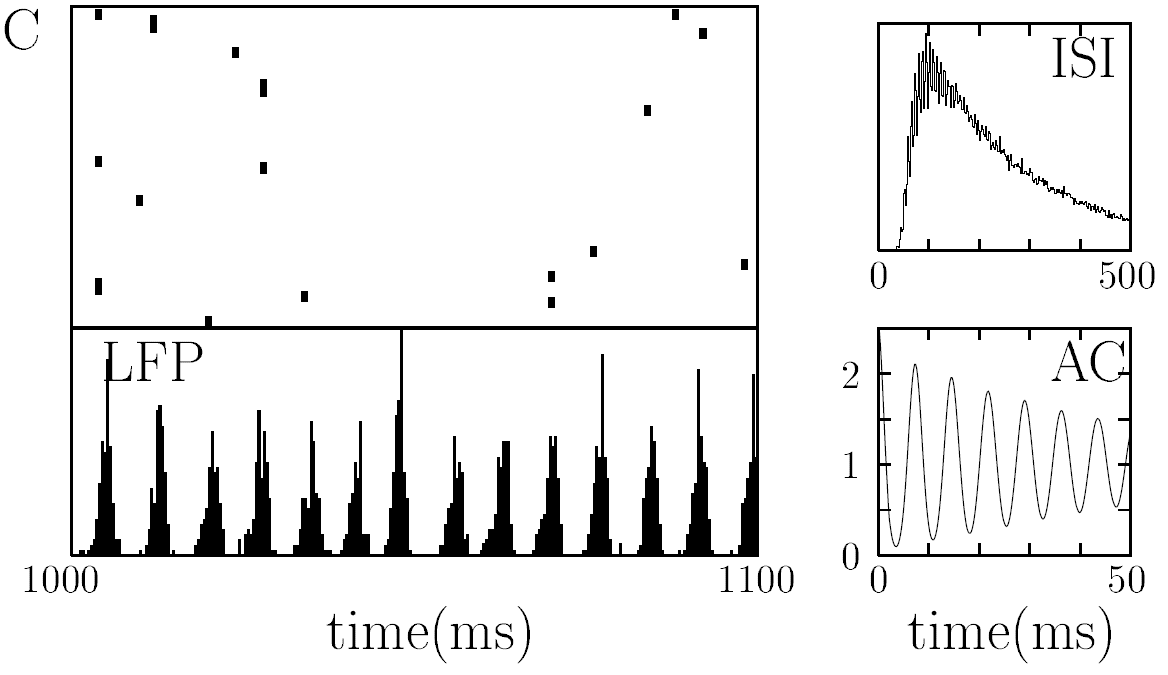
\includegraphics[width=.6\textwidth]{figures/brunel2.png}
  \end{center}
  \begin{flushright}
    {\footnotesize Brunel \& Hakim 1999}
   \end{flushright}
\end{frame}

\subsection{Non-random connectivity}

\begin{frame}{Random is not enough (I)}
    \begin{itemize}
      \item Distance dependent connectivity
    \end{itemize}
    \vspace*{.5cm}
    \begin{minipage}{.28\linewidth}
  \begin{center}
	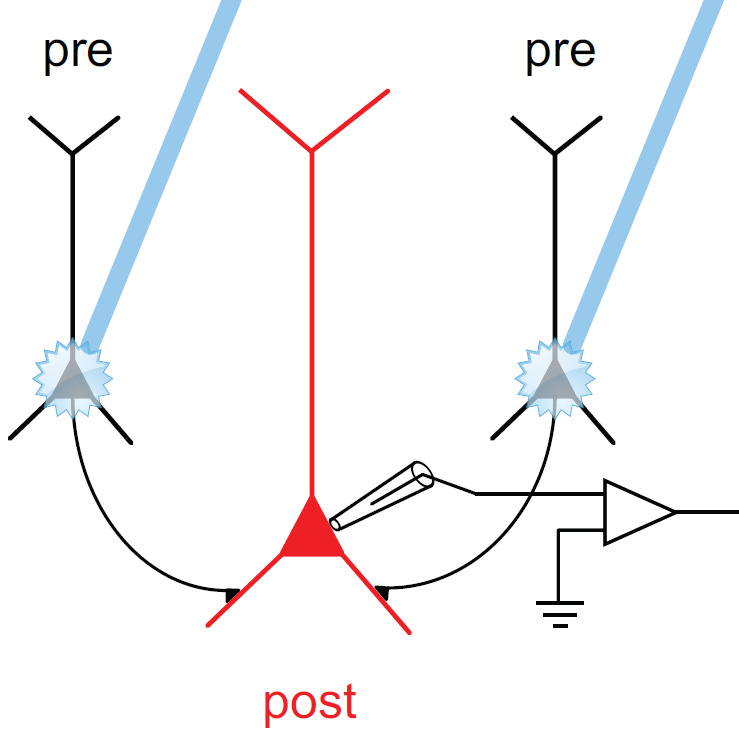
\includegraphics[width=\linewidth]{figures/boucsein0.png}
  \end{center}
    \begin{flushright}
	{\footnotesize \cite{Boucsein2011}}
    \end{flushright}
    \end{minipage}\ppc{5}
        \begin{minipage}{.68\linewidth}
  \begin{center}
	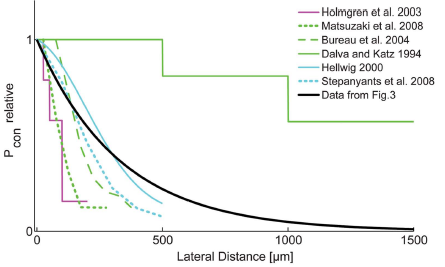
\includegraphics[width=.9\linewidth]{figures/boucsein1.png}
  \end{center}
      \end{minipage}
\end{frame}

\begin{frame}{Random is not enough (II)}
    \begin{itemize}
      \item Highly non-random distribution of connectivity motifs
    \end{itemize}
    \vspace*{.5cm}
    \begin{minipage}{.38\linewidth}
    \begin{center}
	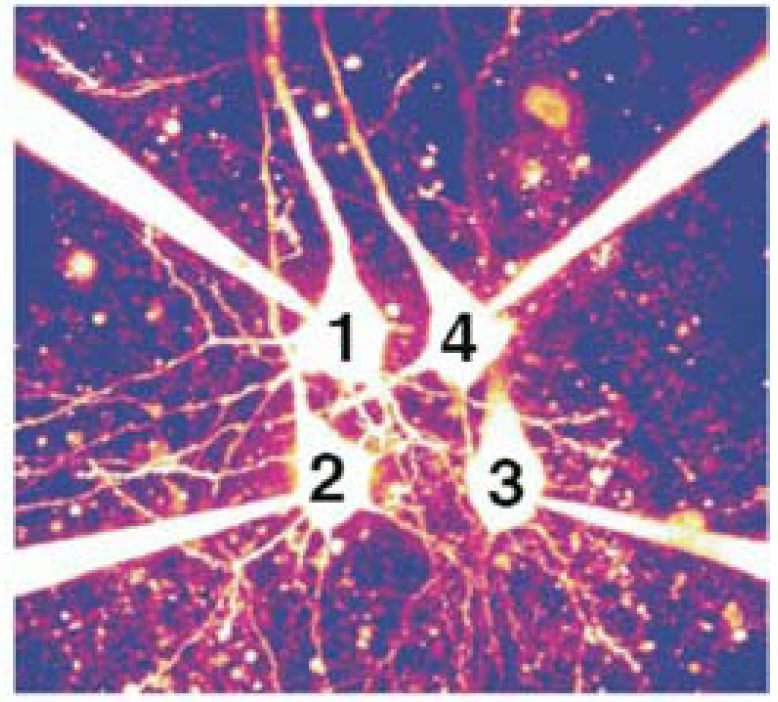
\includegraphics[width=.8\linewidth]{figures/song0.png}
    \end{center}
    \begin{flushright}
	{\footnotesize \cite{Song2005}}
    \end{flushright}
    \end{minipage}\ppc{6}
    \begin{minipage}{.58\linewidth}
    \begin{center}
	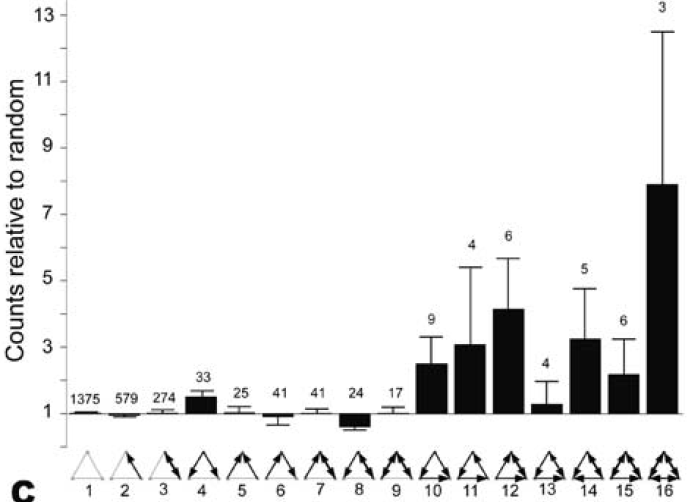
\includegraphics[width=.8\linewidth]{figures/song1.png}
    \end{center}
    \end{minipage}
\end{frame}



\section{Effect of topology on network dynamics}

\subsection{Degree distribution}

\begin{frame}{Degree distribution}
  \begin{itemize}
    \item The width of the in-degree distribution determines the level of
synchrony in the network.
  \end{itemize}\ppc{7}
  \vspace*{.2cm}
\begin{minipage}{.48\linewidth}
\textcolor{red}{Inh}
    \begin{center}
	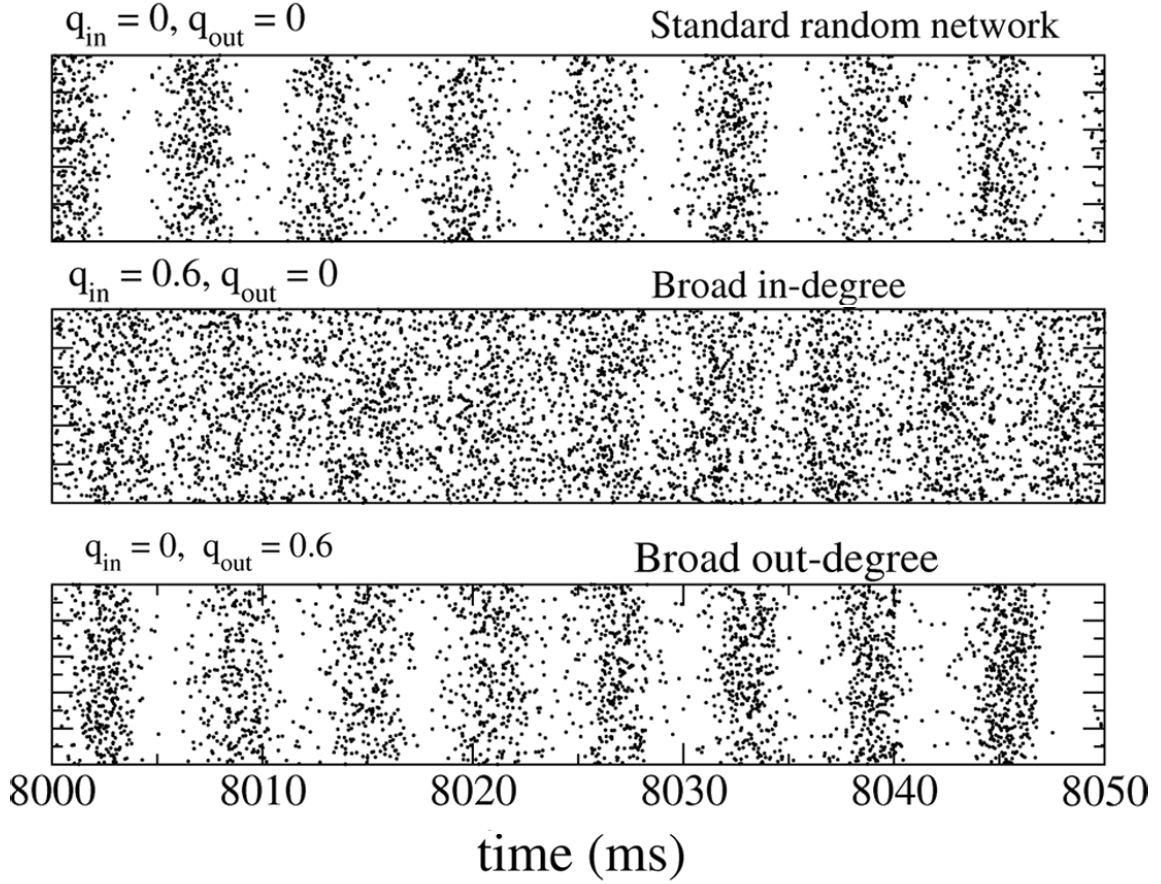
\includegraphics[width=\textwidth]{figures/roxin0}
    \end{center}
\end{minipage}\ppc{7}
\begin{minipage}{.48\linewidth}
    \textcolor{blue}{Exc}-\textcolor{red}{Inh}
    \begin{center}
    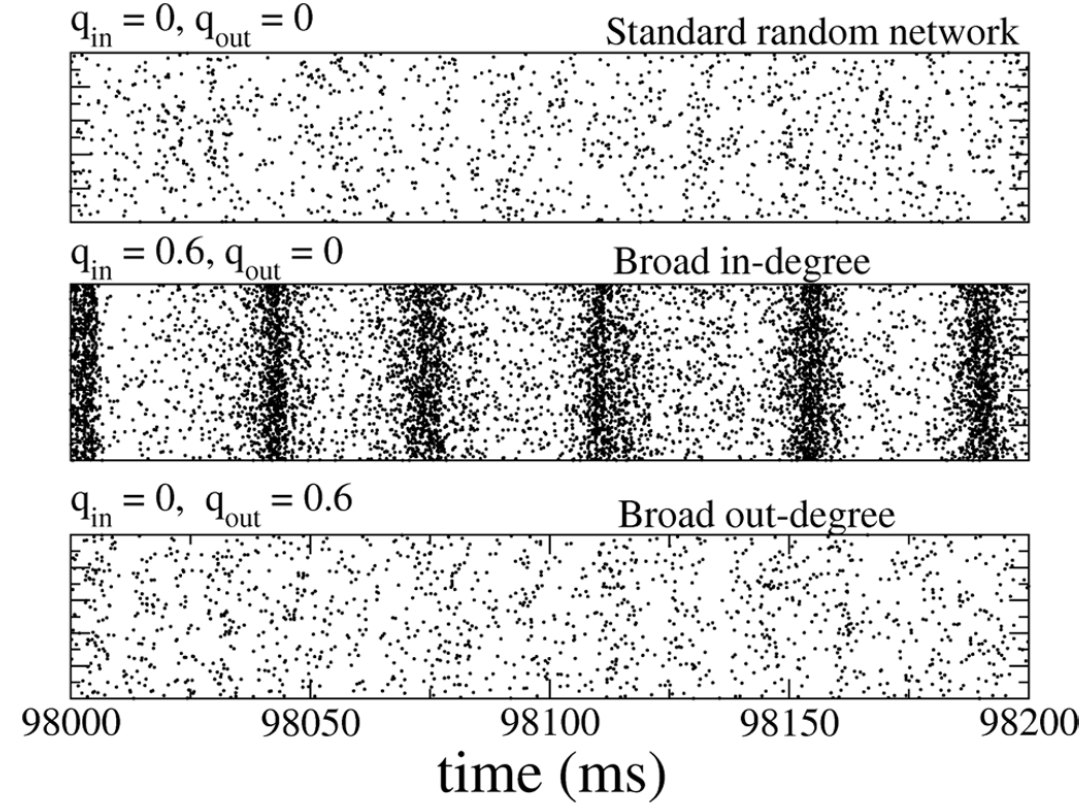
\includegraphics[width=\textwidth]{figures/roxin1}
    \end{center}
\end{minipage}
    \begin{flushright}
      {\footnotesize \cite{Roxin2011}}
    \end{flushright}
\end{frame}

\subsection{Dale versus hybrid connectivity}
\pc{8}

\begin{frame}{Dale versus hybrid connectivity}
  \begin{center}
    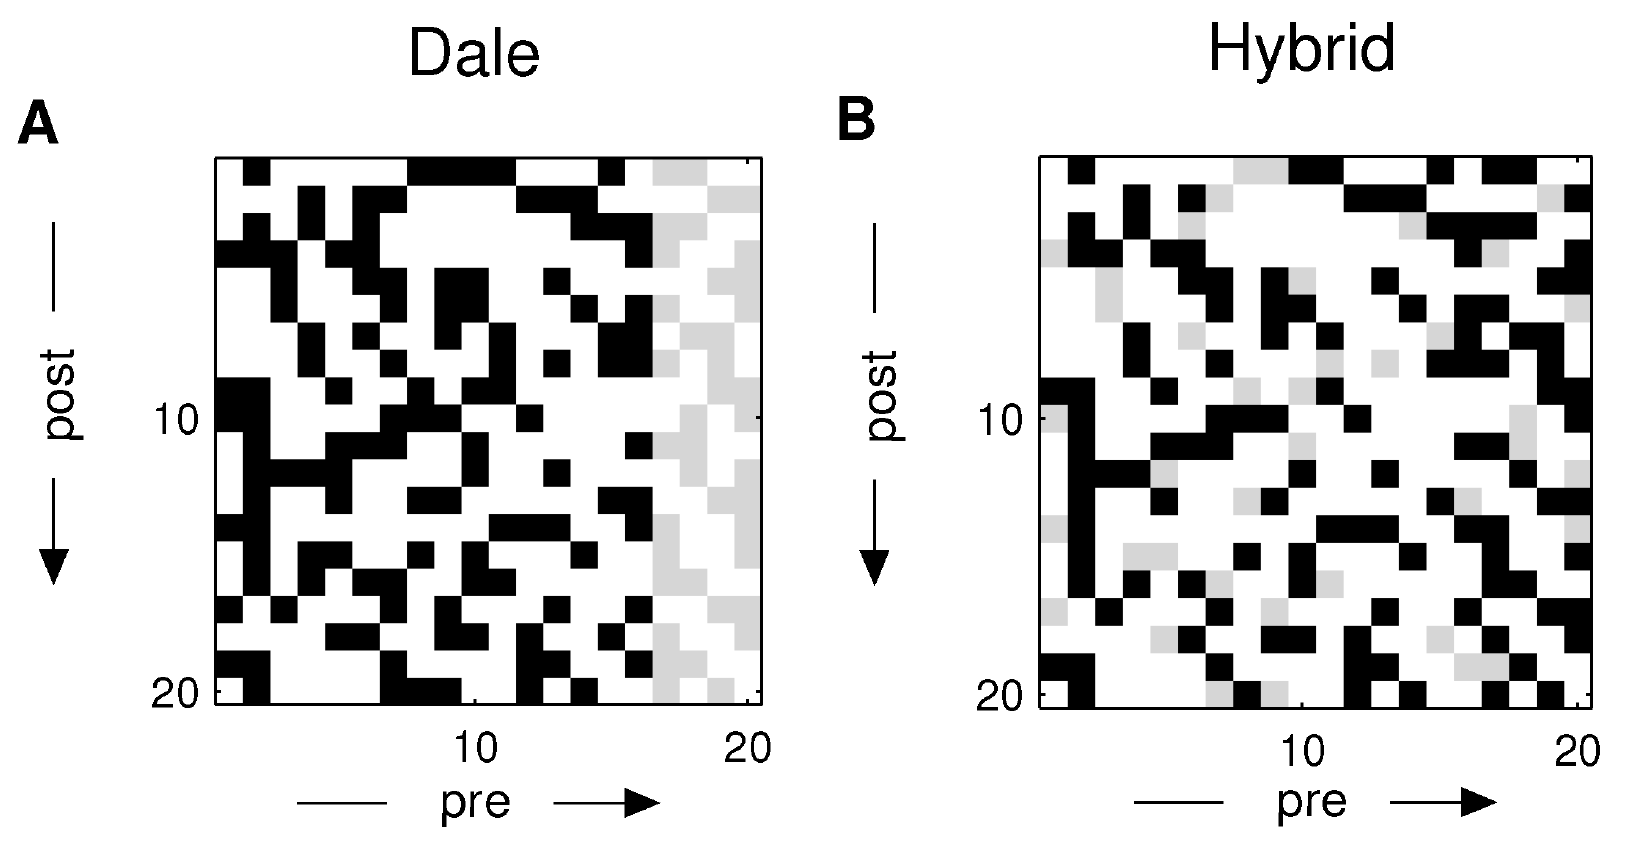
\includegraphics[width=.7\textwidth]{figures/kriener_dale0}
  \end{center}
    \begin{flushright}
      {\footnotesize \cite{Kriener2008}}
    \end{flushright}
\end{frame}

\begin{frame}{Dale versus hybrid connectivity}
  \begin{minipage}{.48\linewidth}
   \begin{center}
\hspace*{-0.2cm}
    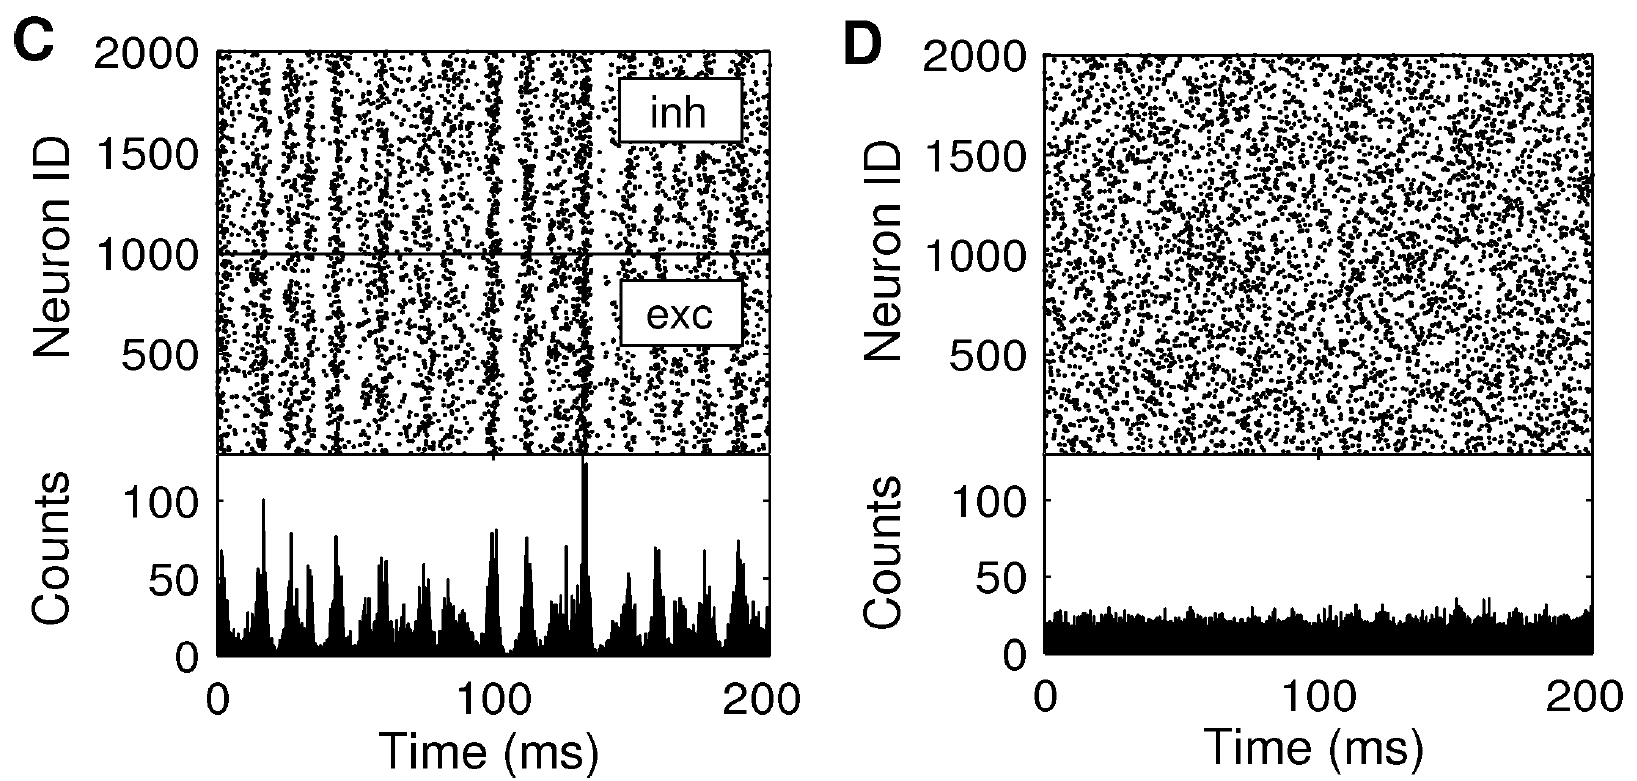
\includegraphics[width=\textwidth]{figures/kriener_dale1}
   \end{center}
  \end{minipage}\ppc{9}
\begin{minipage}{.48\linewidth}
 \begin{center}
\hspace*{0.25cm}
    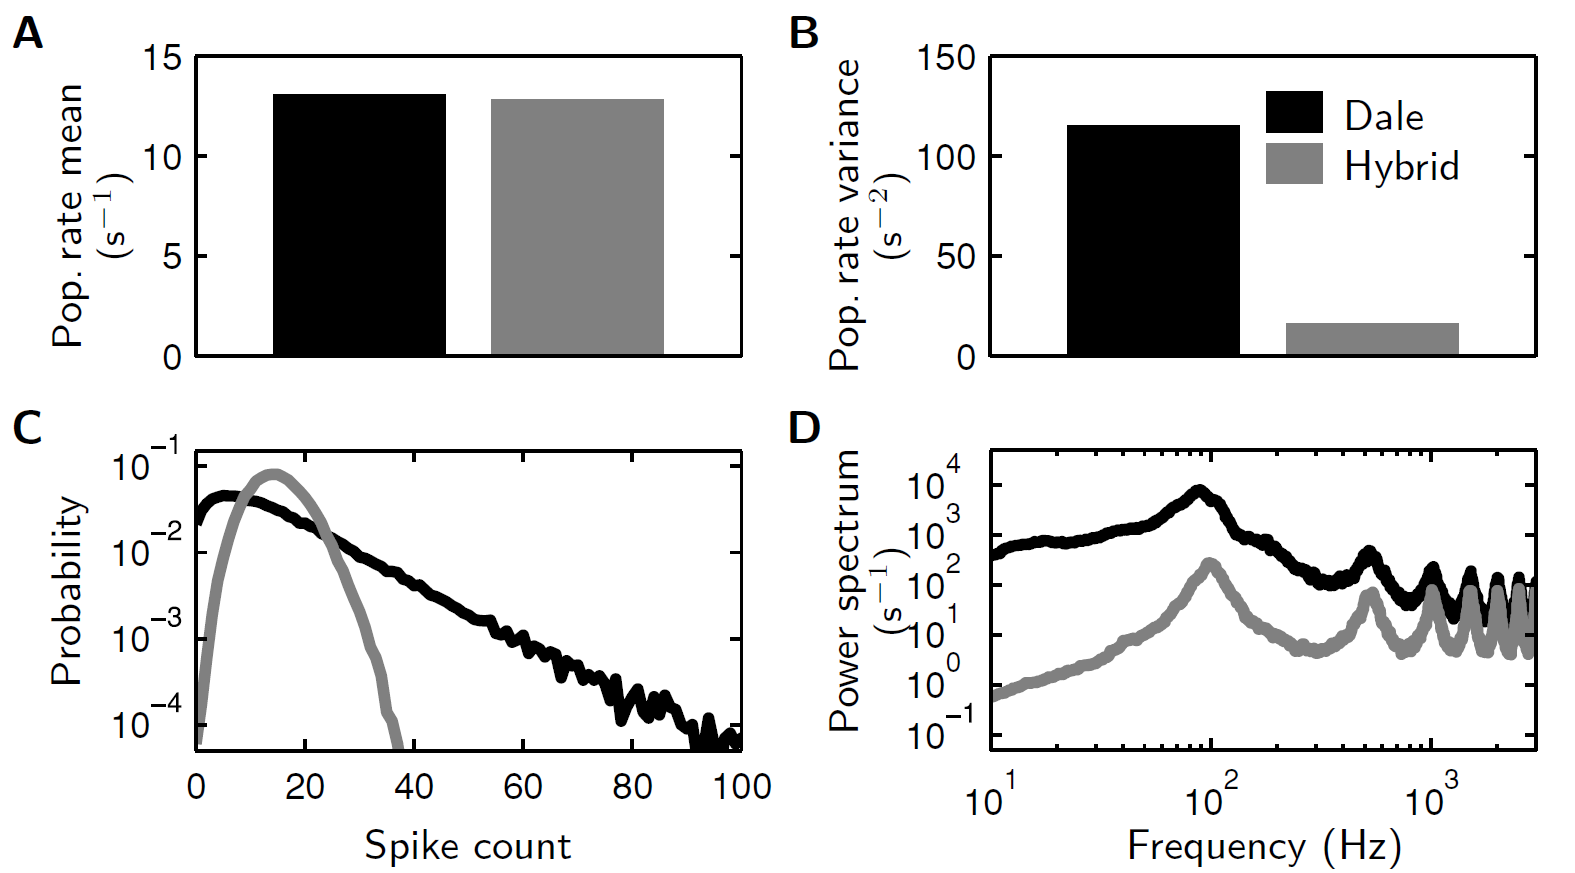
\includegraphics[scale=0.11]{figures/kriener_dale2}
 \end{center}
     \begin{flushright}
      {\footnotesize \cite{Kriener2008}}
    \end{flushright}
\end{minipage}
\vspace*{1cm}
    \begin{itemize}
      \item Same mean firing rate
      \item Hybrid less synchronous than Dale
    \end{itemize}
\end{frame}

\subsection{Distance dependent connectivity}


\begin{frame}{Distance dependent connectivity}
  \begin{center}
    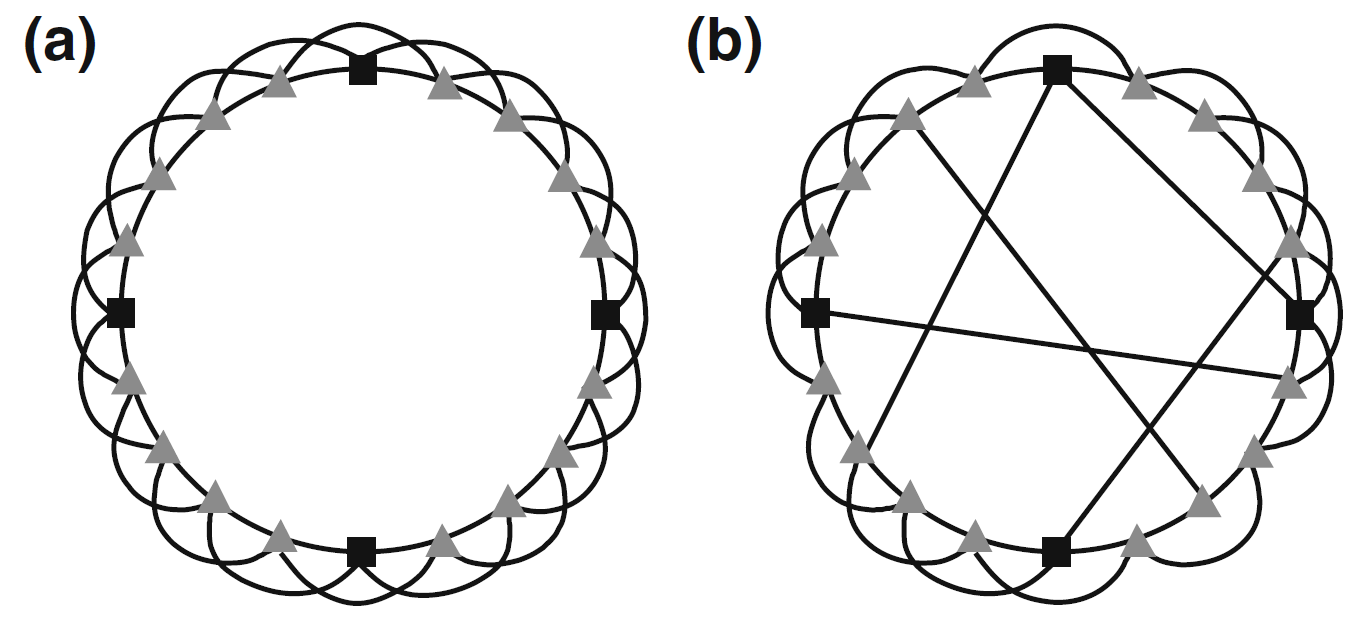
\includegraphics[width=.6\textwidth]{figures/kriener_dist1a}
  \end{center}
    \begin{flushright}
      {\footnotesize \cite{Kriener2009}}
    \end{flushright}
    \begin{itemize}
     \item Probability of rewiring ${\mathrm{p_r}}$\ppc{10}
     \item $0<{\mathrm{p_r}}<1$ $\rightarrow$ \curldoquom{small-world} network
({\footnotesize \cite{Watts1998}})
    \end{itemize}
\end{frame}


\begin{frame}{Distance dependent connectivity}
  \begin{minipage}{.38\linewidth}
   \begin{center}
    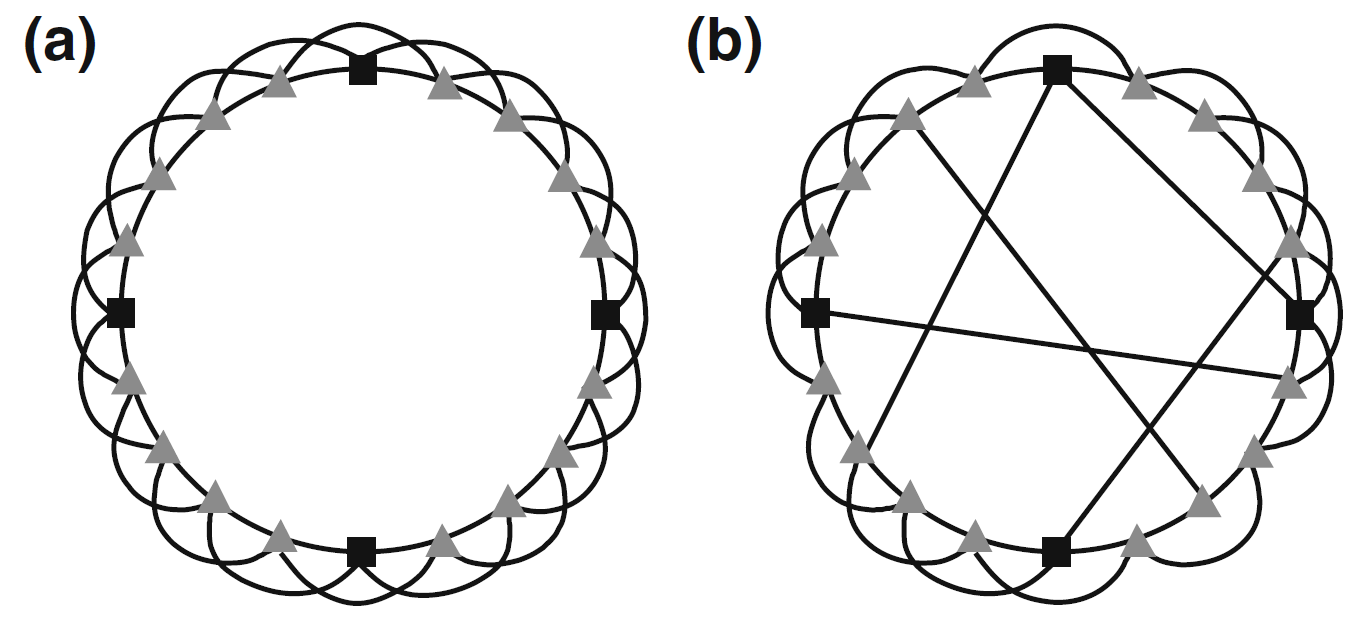
\includegraphics[width=.9\textwidth]{figures/kriener_dist1a}
   \end{center}
        \begin{flushright}
      {\footnotesize \cite{Kriener2009}}
    \end{flushright}
  \end{minipage}\ppc{11}
\begin{minipage}{.58\linewidth}
 \begin{center}
    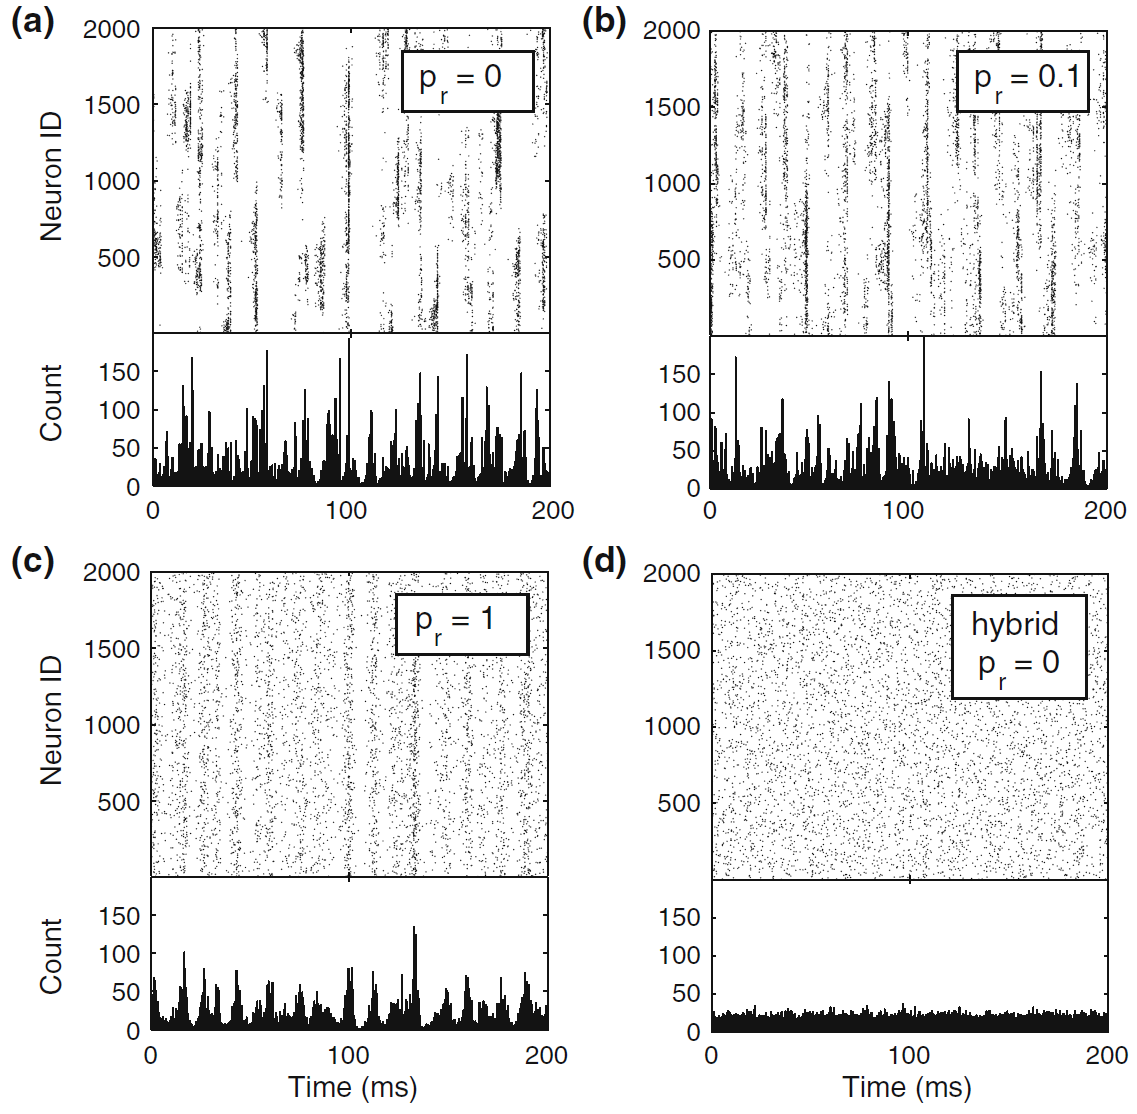
\includegraphics[width=.9\textwidth]{figures/kriener_dist2}
 \end{center}
 \vspace*{.2cm}
\end{minipage}
    \begin{itemize}
      \item Clustered networks are \curldoquom{locally} more synchronous.
      \item Hybrid beats local connectivity!
    \end{itemize}
\end{frame}

\subsection{Clustered networks and metastability}


\begin{frame}{Clustered networks and metastability}
   \begin{minipage}{.48\linewidth}
   \begin{center}
	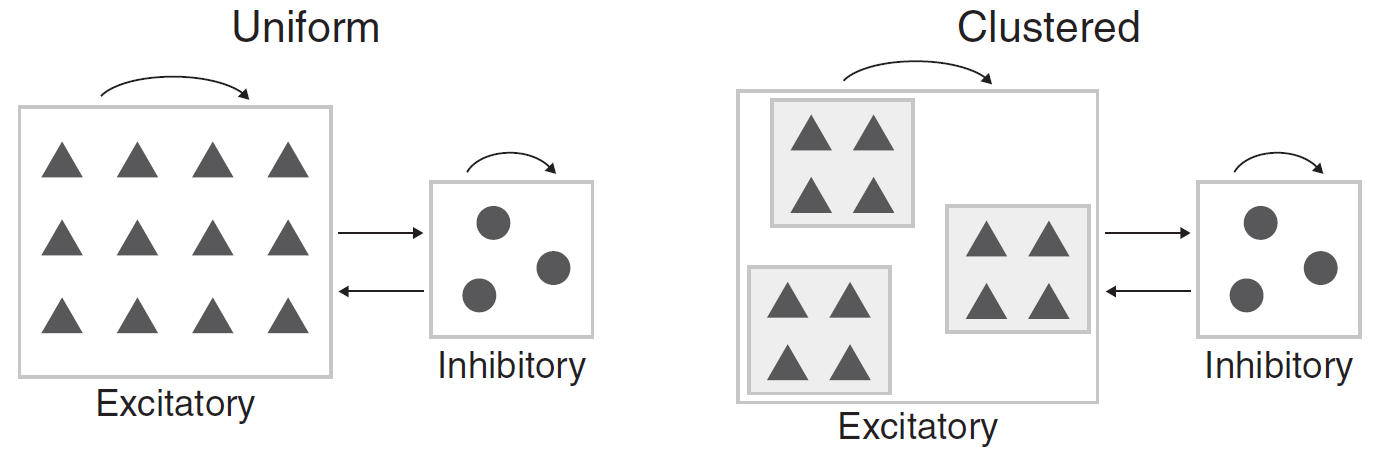
\includegraphics[width=\textwidth]{figures/doiron3}
	\vspace*{.1cm}
	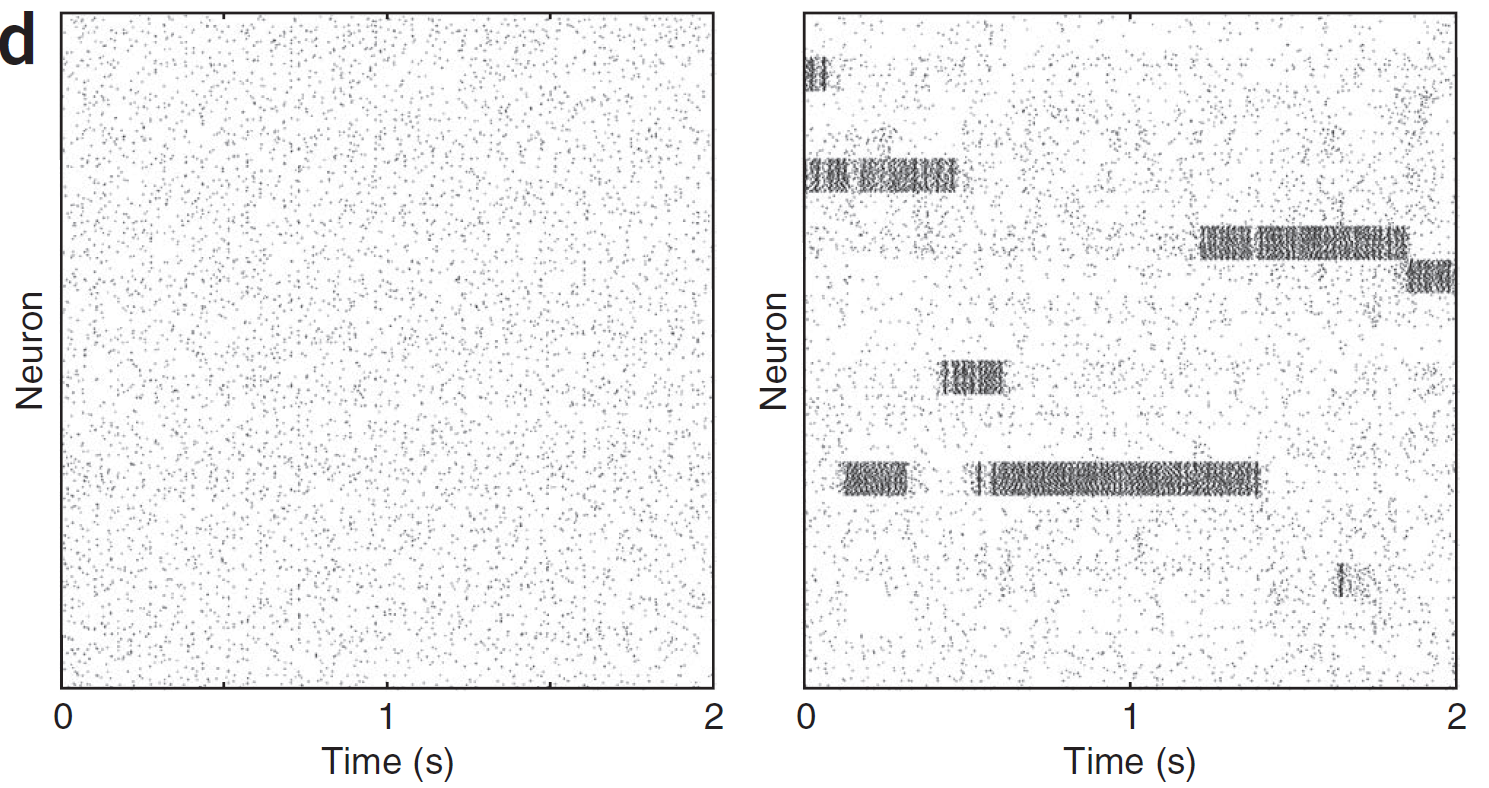
\includegraphics[width=\textwidth]{figures/doiron4}  
    \end{center}
        \begin{flushright}
      {\footnotesize \cite{Litwin-Kumar2012}}
    \end{flushright}
  \end{minipage}\ppc{12}
\begin{minipage}{.48\linewidth}
 \begin{center}
    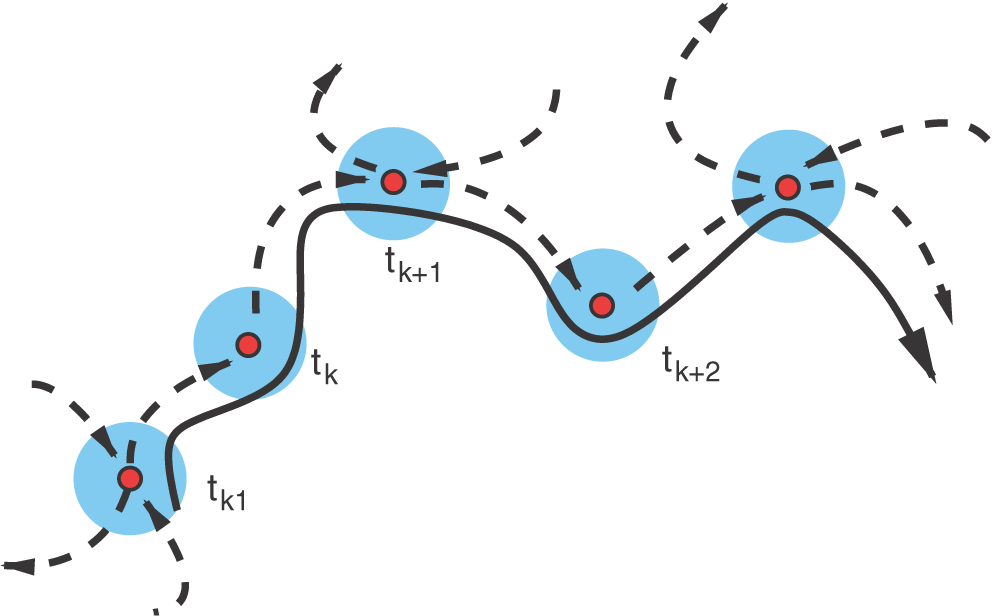
\includegraphics[width=.9\textwidth]{figures/rabinovich1}
        \begin{flushright}
        \vspace*{-.3cm}
      {\footnotesize Rabinovich et al. 2008}
    \end{flushright}\ppc{12}
    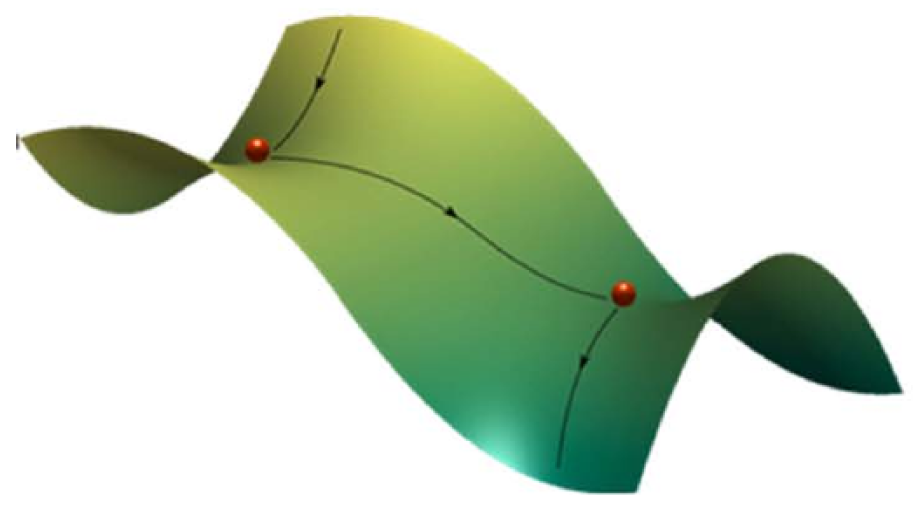
\includegraphics[width=.9\textwidth]{figures/rabinovich2}
        \begin{flushright}
      {\footnotesize Rabinovich \& Varona 2011}
    \end{flushright}
    \end{center}
 \vspace*{.2cm}
\end{minipage}
\end{frame}


\section{Applications to real data}

\subsection{Stimulus induced variability reduction}

\pc{13}
\begin{frame}{Stimulus-induced variability reduction}
  \begin{center}
     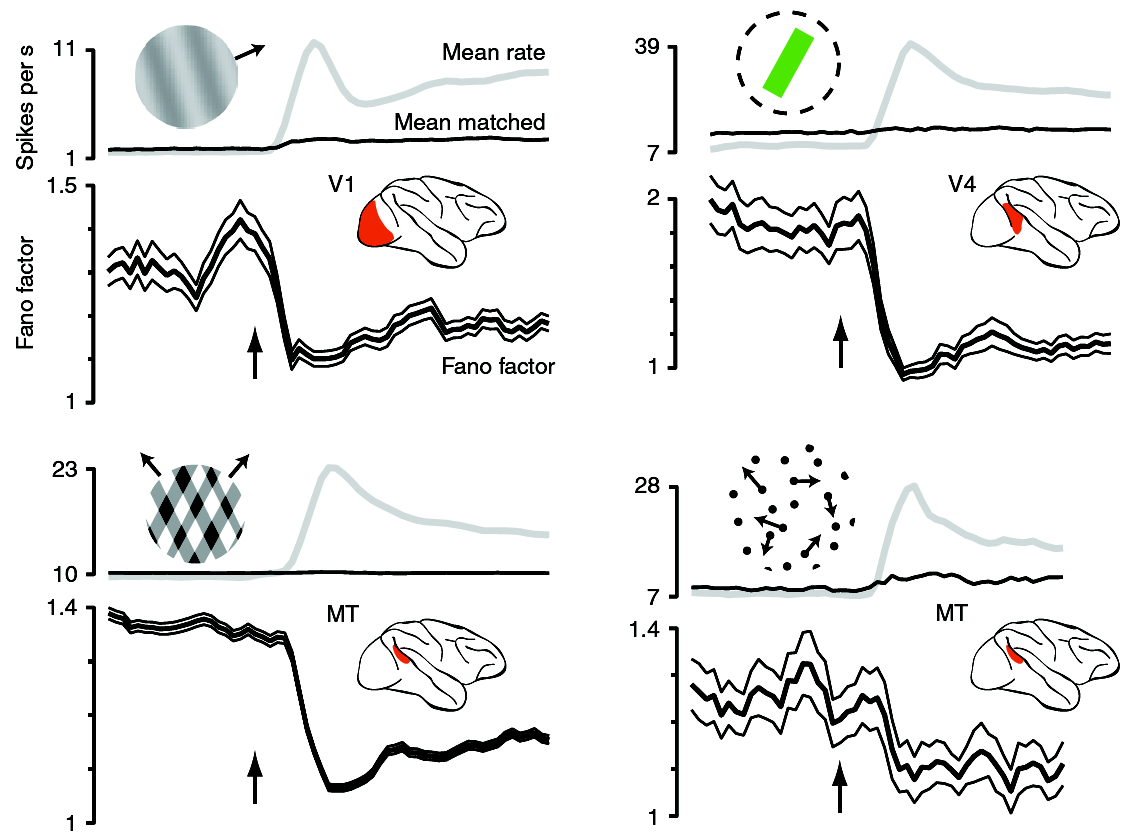
\includegraphics[width=.7\textwidth]{figures/churchland1}
  \end{center}
    \begin{flushright}
	{\footnotesize \cite{Churchland2010}}
    \end{flushright}
\end{frame}

\begin{frame}{Stimulus-induced variability reduction}
\begin{minipage}{.48\linewidth}
 \begin{center}
	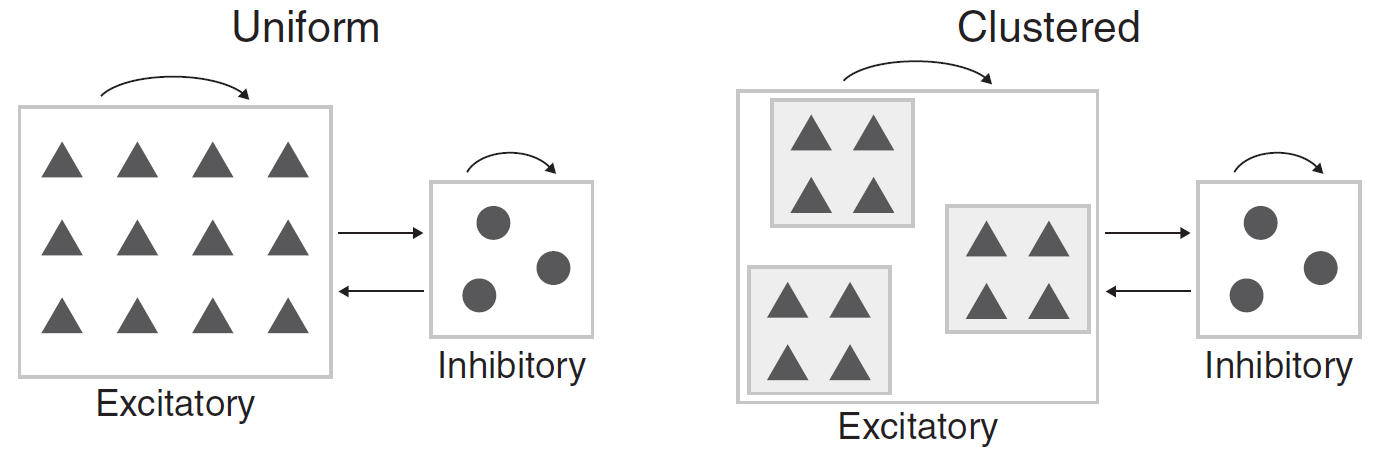
\includegraphics[trim=7cm 0cm 0cm
0cm,clip=true,width=.8\textwidth]{figures/doiron3}
 \end{center}
 \begin{center}
	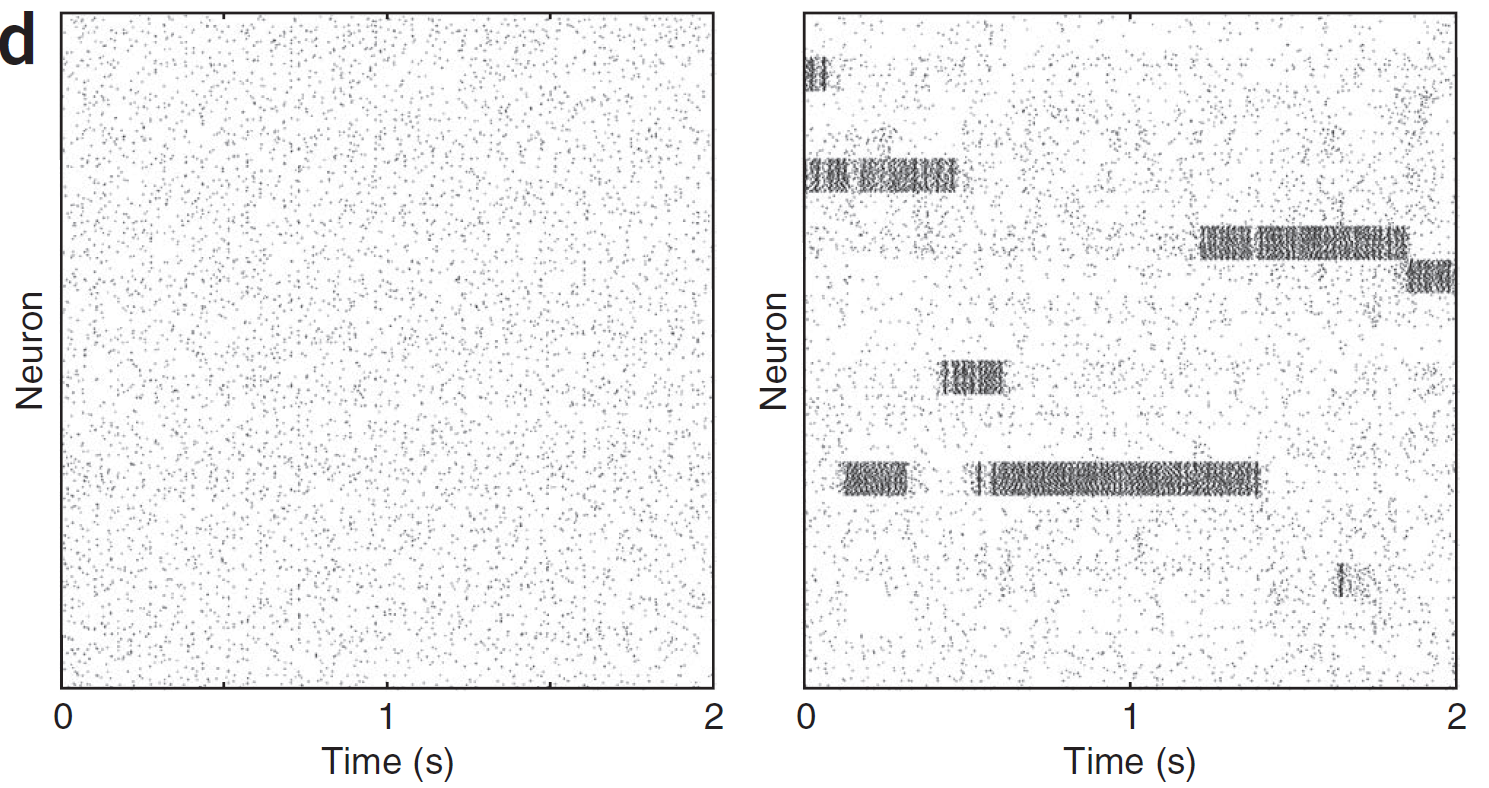
\includegraphics[trim=7.6cm 0cm 0cm
0cm,clip=true,width=.8\textwidth]{figures/doiron4}
 \end{center}
\end{minipage}\ppc{14}
\begin{minipage}{.48\linewidth}
 \begin{center}
  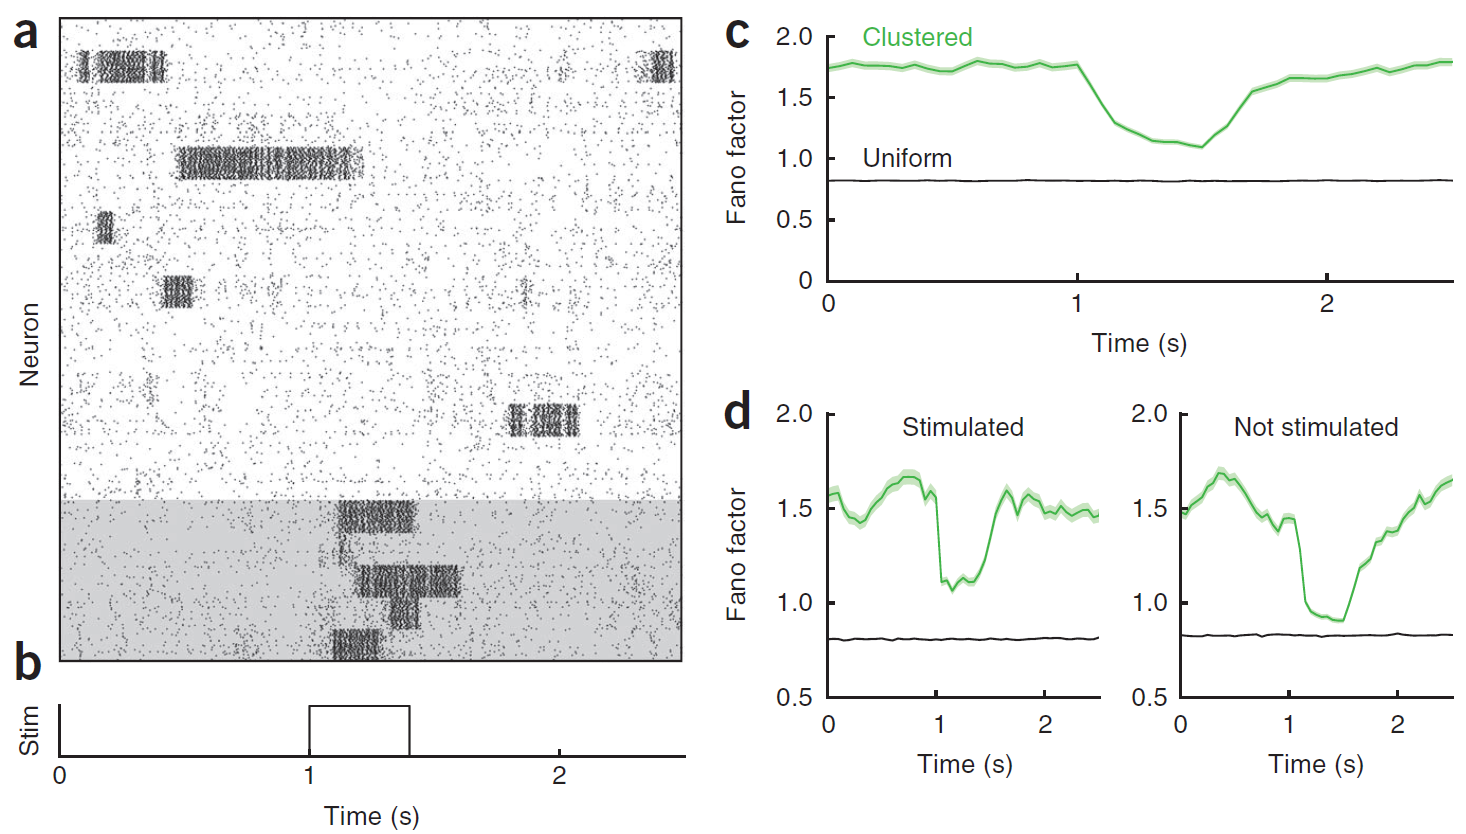
\includegraphics[width=6cm,keepaspectratio=true]{figures/doiron2}
  \begin{flushright}
      {\footnotesize \cite{Litwin-Kumar2012}}
  \end{flushright}
\end{center}
\end{minipage}
\end{frame}

\subsection{Complex spatio-temporal dynamics during reaching}

\begin{frame}{Neural dynamics during reaching}
\begin{itemize}
 \item Neurons in motor cortex produce complex spatio-temporal patterns during
reaching movements.
\end{itemize}\ppc{15}
 \begin{minipage}{.48\linewidth}
 \begin{center}
	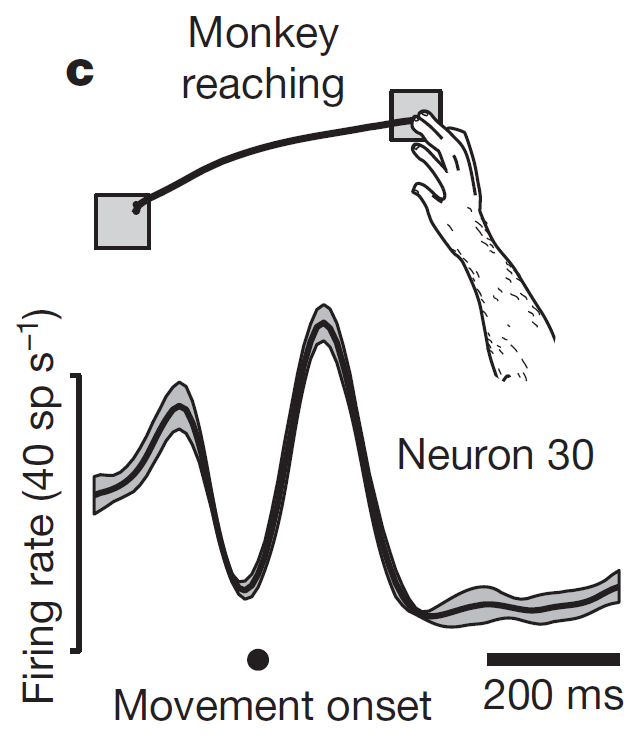
\includegraphics[width=.7\textwidth]{figures/churchland3}
  \begin{flushright}
      {\footnotesize \cite{Churchland2012}}
  \end{flushright}
\end{center}
\end{minipage}\ppc{15}
\begin{minipage}{.48\linewidth}
 \begin{center}
	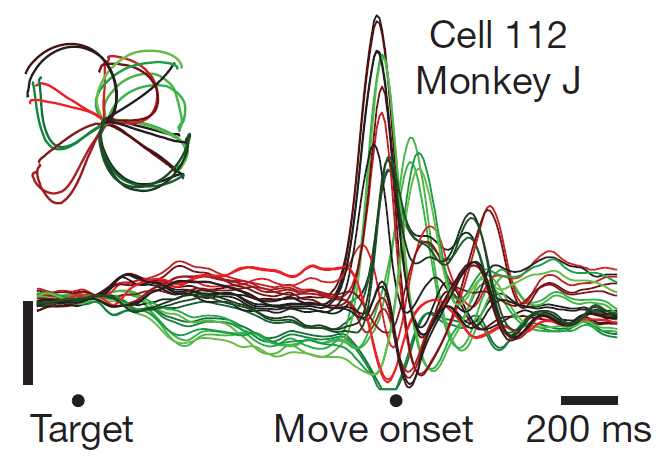
\includegraphics[width=.7\textwidth]{figures/churchland4}
\end{center}
\end{minipage}
\end{frame}

\begin{frame}{Detailed balance connectivity}
 \begin{itemize}
  \item \curldoquom{Detailed balance} connectivity stabilizes the network
dynamics.
 \end{itemize}\ppc{16}
 \vspace*{1cm}
 \begin{minipage}{.48\linewidth}
 \begin{center}
  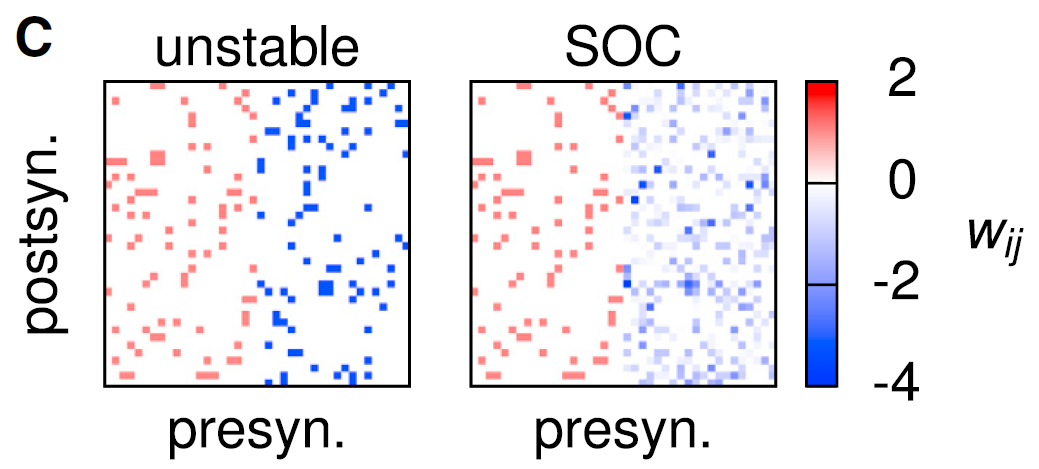
\includegraphics[width=\textwidth]{figures/hennequin1}
  \begin{flushright}
  {\footnotesize \cite{Hennequin2014}}
\end{flushright}
\end{center}
\end{minipage}\ppc{16}
\begin{minipage}{.48\linewidth}
 \begin{center}
  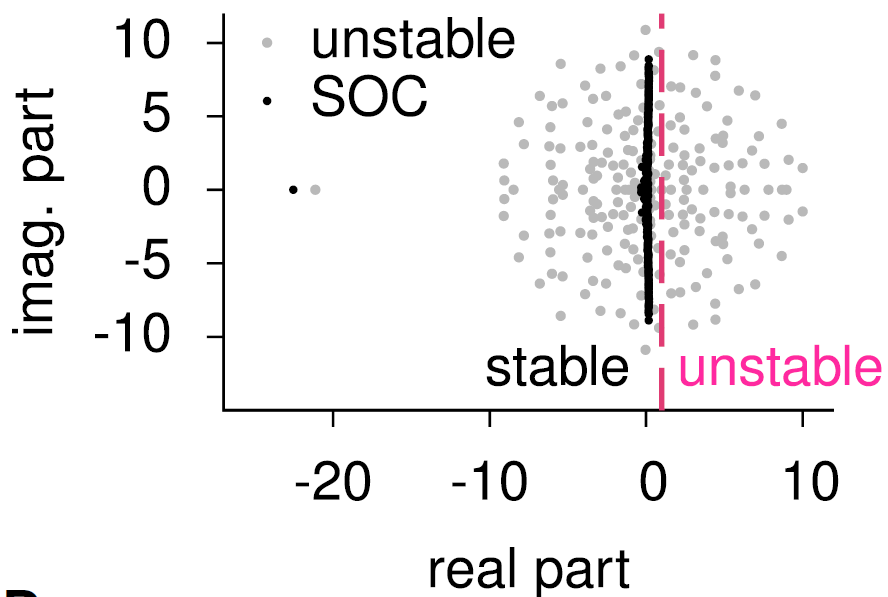
\includegraphics[width=.8\textwidth]{figures/hennequin2}
\end{center}
\end{minipage}
\end{frame}


\begin{frame}{Detailed balance connectivity}
 \begin{itemize}
  \item \curldoquom{Detailed balance} networks can reproduce the complex
spatio-temporal neural activity patterns found in motor cortex.
 \end{itemize}\ppc{17}
\begin{center}
   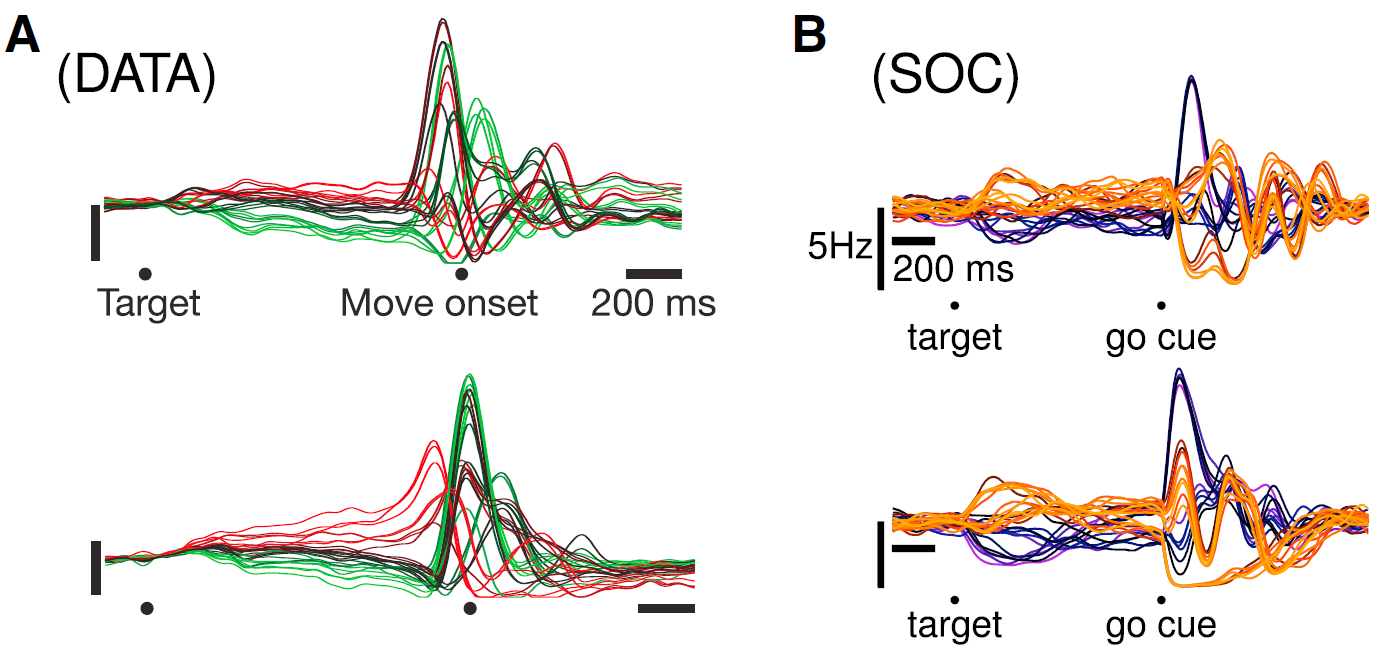
\includegraphics[width=.8\textwidth]{figures/hennequin3}
\end{center}
  \begin{flushright}
  {\footnotesize \cite{Hennequin2014}}
\end{flushright}
\end{frame}

\section{Summary}

\begin{frame}{Summary}

\pc{18}
\begin{itemize}
  \item Random network models can capture many features of cortical activity but
not all.\ppc{18}
  \item Experimental evidence refutes the random connectivity
hypothesis.\ppc{18}
  \item The degree distributions have a strong impact on the level of
synchrony in the network.\ppc{18}
  \item Clustered network can generate \curldoquom{metastable} dynamics that are
highly variable.\ppc{18}
  \item The stimulation of a cluster in a clustered network can reproduce the
stimulus-induced drop in firing rate variability.\ppc{18}
\item A detailed balance connectivity can reproduce the complex
spatio-temporal neural activity patterns found in motor cortex.
\end{itemize}
\end{frame}

\section{Bibliography}
\setcounter{page}{18}
\begin{frame}{Bibliography (I)}
\begin{thebibliography}{9}

\bibitem[Pernice et al. 2011]{Pernice2011}
Pernice, V and Staude, B and Cardanobile, S and Rotter, S
\newblock How structure determines correlations in neuronal networks
\newblock {\em PLoS Computat Biol}, 7(5), 2011

\bibitem[Kriener et al., 2008]{Kriener2008}
Kriener, B and Tetzlaff, T and Aertsen, A and Diesmann, M and  Rotter, S
\newblock Correlations and population dynamics in cortical networks
pathways and memory networks
\newblock {\em Neural Comput}, 20(9):2185-2226, 2008

\bibitem[Kriener et al., 2009]{Kriener2009}
Kriener, B and Helias, M and Aertsen, A and Rotter, S
\newblock Correlations in spiking neuronal networks with distance dependent
connections
\newblock {\em J Comput Neurosci}, 27(2):177-200, 2009

\end{thebibliography}
\end{frame}
\setcounter{page}{18}
\begin{frame}{Bibliography (II)}
\begin{thebibliography}{9}

\bibitem[Watts \& Strogatz, 1998]{Watts1998}
Watts, D J and Strogatz, S H
\newblock Collective dynamics of \curldoquom{small-world} networks
\newblock {\em Nature}, 393(6684):440-442, 1998

\bibitem[Litwin-Kumar \& Doiron, 2012]{Litwin-Kumar2012}
Litwin-Kumar, A and Doiron, B
\newblock Slow dynamics and high variability in balanced cortical networks with
clustered connections
\newblock {\em Nature Neurosci}, 15(11):1498-1505, 2012


\bibitem[Doiron \& Litwin-Kumar, 2014]{Doiron2014}
Doiron, B and Litwin-Kumar, A 
\newblock Balanced neural architecture and the idling brain
\newblock {\em Front Comput Neurosci}, 8. 2014



\end{thebibliography}
\end{frame}

\setcounter{page}{18}
\begin{frame}{Bibliography (III)}
\begin{thebibliography}{9}

 \bibitem[Hennequin et al., 2014]{Hennequin2014}
Hennequin, G and Vogels, T P and Gerstner, W
\newblock Optimal control of transient dynamics in balanced networks
supports generation of complex movements
\newblock  {\em Neuron}, 82(6):1394-1406, 2014

\bibitem[Churchland et al. 2012]{Churchland2012}
Churchland, M M and Cunningham, J P,  ... and Shenoy, K V
\newblock Neural population dynamics during reaching 
\newblock {\em Nature}, 2012

\bibitem[Churchland et al. 2010]{Churchland2010}
Churchland, M M, Byron, M Y, ... and Shenoy, K V
\newblock Stimulus onset quenches neural variability: a widespread cortical
phenomenon 
\newblock {\em Nature Neurosci}, 13(3):369-378, 2010

\end{thebibliography}

\end{frame}

\setcounter{page}{18}
\begin{frame}{Bibliography (IV)}
\begin{thebibliography}{9}

 \bibitem[Roxin, 2011]{Roxin2011}
Roxin, A
\newblock The role of degree distribution in shaping the dynamics in
networks of sparsely connected spiking neurons
\newblock  {\em Front Comput Neurosci}, 5, 2011

\bibitem[Boucsein et al. 2011]{Boucsein2011}
Boucsein, C and Nawrot, M and Schnepel, P and Aertsen, A
\newblock Beyond the cortical column: abundance and physiology of horizontal
connections imply a strong role for inputs from the surround
\newblock {\em Front Neurosci}, 5(322), 2011

\bibitem[Song et al. 2005]{Song2005}
Song, S and Sj\"{o}str\"{o}m, P J and Reigl, M and Nelson, S and Chklovskii, D
B
\newblock Highly nonrandom features of synaptic connectivity in local cortical
circuits 
\newblock {\em PLoS Biol}, 3(3), e68, 2005

\end{thebibliography}

\end{frame}


\end{document}

